\documentclass[11pt, twoside]{article} %iniciación del documento de tipo artículo, con tamaño de letra 11pt.
\usepackage[a4paper,total={6in, 8in},left=25mm, asymmetric]{geometry} %Cambio en los bordes y margenes del documento

\usepackage{fancyhdr} %Paquete para organizar y añadir header con los nombres

\usepackage{amsmath}

\usepackage[spanish,es-tabla,es-nodecimaldot]{babel}
\usepackage{tabularx}
\usepackage{booktabs}

\usepackage{caption}

\usepackage{graphicx}
\usepackage[hidelinks]{hyperref}
\usepackage{macro}

\fancypagestyle{main}{
    \fancyhf{}
    \fancyhead[L]{\thepage}
    \fancyhead[RO]{Z. Liu}
    \renewcommand{\headrulewidth}{.4pt}
    \setlength{\headheight}{52pt}
}

\pagestyle{empty}

\begin{document}

\begin{figure}[h!]
    \minipage{0.87\textwidth}
	
\includegraphics[width=3cm]{Icons/ugr.jpg}
	\endminipage
    \minipage{0.87\textwidth}
	
\includegraphics[height = 2.5cm, width=3cm]{Icons/facultad_ciencias.png}
	\endminipage
	%%\vspace{-1cm}
\end{figure}

\vspace{0.3cm}

\begin{center}
    \Huge \textbf{Física Computacional}\\
    		\vspace{0.4cm}
    \LARGE \textbf{Voluntario 2:}  
    Estudio del péndulo doble con un algoritmo Runge-Kutta.
\end{center}

\vspace{1cm}

\vspace{1cm}

\begin{center}
    \large \textbf{Resumen}\\
    		\vspace{0.2cm}
    \normalsize
    En este informe tenemos como objetivo estudiar el comportamiento del 
    doble pendulo, empleando el método de Runge-Kutta para simular el
    movimiento del sistema. Se estudiará la relación entre sus variables
    y la energía total del sistema, para distintas condiciones iniciales.
    Además se analizará la estabilidad del sistema y la influencia pequeñas 
    perturbaciones.

\end{center}

\vspace{1cm}

\begin{flushright}
    \large ZhuoZhuo Liu 
    \\
    \vspace{0.4cm}
    \textbf{Grado en Física}
\end{flushright}

\newpage

\setcounter{page}{0}
\tableofcontents
\newpage

\pagestyle{main}

\section{Introducción}

\section{Planteamiento del problema}
\subsection{Ecuaciones del movimiento}
Primero debemos de hallar las expresiones de los momentos angulares
a partir del Lagrangiano del sistema. 

\begin{equation}
    \mathcal{L} = \dot{\phi}^2 + \dot{\phi}\dot{\psi} \cos(\psi - \phi) +
     \frac{1}{2}\dot{\psi}^2 - 2g(1-\cos\phi) - g(1-\cos\psi) 
\end{equation}

Hallamos las expresiones del momento angular $p_\phi$ y $p_\psi$, en función
de las velocidades angulares $\dot{\phi}$ y $\dot{\psi}$ através de las 
parciales de $\mathcal{L}$ con respecto a las velocidades angulares.

\begin{equation}
    p_\phi = \frac{\partial \mathcal{L}}{\partial \dot{\phi}} = 2\dot{\phi} + \dot{\psi}\cos(\psi - \phi)
\end{equation}

\begin{equation}
    p_\psi = \frac{\partial \mathcal{L}}{\partial \dot{\psi}} = \dot{\psi} + \dot{\phi}\cos(\psi - \phi)
\end{equation}

Despejando las velocidades en función del momento, permite expresar el 
Hamiltoniano en función de dichos momentos.

\begin{equation}
    \dot{\phi} = \frac{p_\phi - p_\psi\cos(\psi - \phi)}{2-\cos^2(\psi - \phi)}, \quad 
    \dot{\psi} = \frac{2p_\psi - p_\phi\cos(\psi - \phi)}{2-\cos^2(\psi - \phi)}
\end{equation}

\begin{equation}
    \begin{split}
        H &= \dot{\phi}^2 + \dot{\phi}\dot{\psi} \cos(\psi - \phi) +
\frac{1}{2}\dot{\psi}^2 + 2g(1-\cos\phi) + g(1-\cos\psi)  \\
 &=\frac{p_\phi^2 + p_\psi^2 - 2p_\phi p_\psi \cos(\psi - \phi)}{2-\cos^2(\psi - \phi)} + 2g(1-\cos\phi) + g(1-\cos\psi)
    \end{split}
\end{equation}

De donde se obtiene las ecuaciones de movimiento a partir de las 
ecuaciones de Hamilton.

\begin{equation}
        \dot{\phi} = \frac{\partial H}{\partial p_\phi} = \frac{p_\phi - p_\psi\cos(\psi - \phi)}{2-\cos^2(\psi - \phi)} 
\end{equation}

\begin{equation}
    \dot{\psi} = \frac{\partial H}{\partial p_\psi} = \frac{2p_\psi - p_\phi\cos(\psi - \phi)}{2-\cos^2(\psi - \phi)}
\end{equation}

\begin{equation}
    \dot{p_\phi} = -\frac{\partial H}{\partial \phi} =  \frac{p_\phi p_\psi \cos^2(\psi - \phi) - (2p_\psi^2 + p_\phi^2)\cos(\psi - \phi) + 2p_\phi p_\psi }{(2-\cos^2(\psi - \phi))^2}2\sin(\phi - \psi) -2g\sin\phi
\end{equation}

\begin{equation}
    \dot{p_\psi} = -\frac{\partial H}{\partial \psi} =  \frac{p_\phi p_\psi \cos^2(\psi - \phi) - (2p_\psi^2 + p_\phi^2)\cos(\psi - \phi) + 2p_\phi p_\psi }{(2-\cos^2(\psi - \phi))^2}2\sin(\psi - \phi) -g\sin\psi
\end{equation}

\subsection{Condiciones iniciales}

Para este tipos de sistemas, las condiciones iniciales son de suma 
importancia para los resultados obtenidos. Tendremos 3 parámetros que tomar
en cuenta, la energía total del sistema y la ángulo inicial de $\phi$ y
$\psi$, ya que se ha considerado $\dot{\psi} (t=0) = 0$ para simplificar.

Depediendo el objetivo del apartado, se irá variando la energía total 
del sistema, los ángulos iniciales, o ambos. Pero es importante tener en
cuenta que la energía total del sistema no puede ser negativa, ya que
la energía potencial es siempre positiva, esto produce ángulos iniciales
incompatibles con la energía propuesta. De modo que para los estudios donde
se varíe la energía, emplearemos ángulos iniciales relativamente pequeños, 
para que sea compatible con la menor energía propuesta.

\subsection{Unidades empleadas}

Aunque se podría realizar en unidades arbitrarias, en el análisis 
de los resultados se asumirá que todos los valores mensionados se 
encuentran en el sistema internacional. Se debe de tomar en cuenta que 
en el hamiltoniano no aparece ni la masa ni la longitud de los hilos 
ya que se han considerado que son iguales con valor 1, es decir 1 kg y 
1 m respectivamente. 

Tambien se ha considerado la gravedad terrestre, de modo que 
$g = 9.81 \text{m/s}^2$. Y para el resto de variables tendrán las 
siguientes unidades:

\begin{itemize}
    \item $\phi$ y $\psi$ en radianes.
    \item $p_\phi$ y $p_\psi$ en $[\text{kg m}^2/\text{s}]$.
    \item $E$ en $[\text{kg m}^2/\text{s}^2]$, es decir en julios [J].
\end{itemize}

\section{Análisis de resultados}

\subsection{Mapas de Poincaré}

Para estudiar el movimiento del sistema, emplearemos los mapas de 
Poincaré para visualizar la relación entre las variables del sistema. 
Comenzando con la relación entre $\phi$ y $\psi$, para distintas 
energías (E = 1, 3, 5, 10, 15). Obteniendo la figura 
\ref{fig:poincare_energias}.

\begin{figure}[h!]
    \centering
    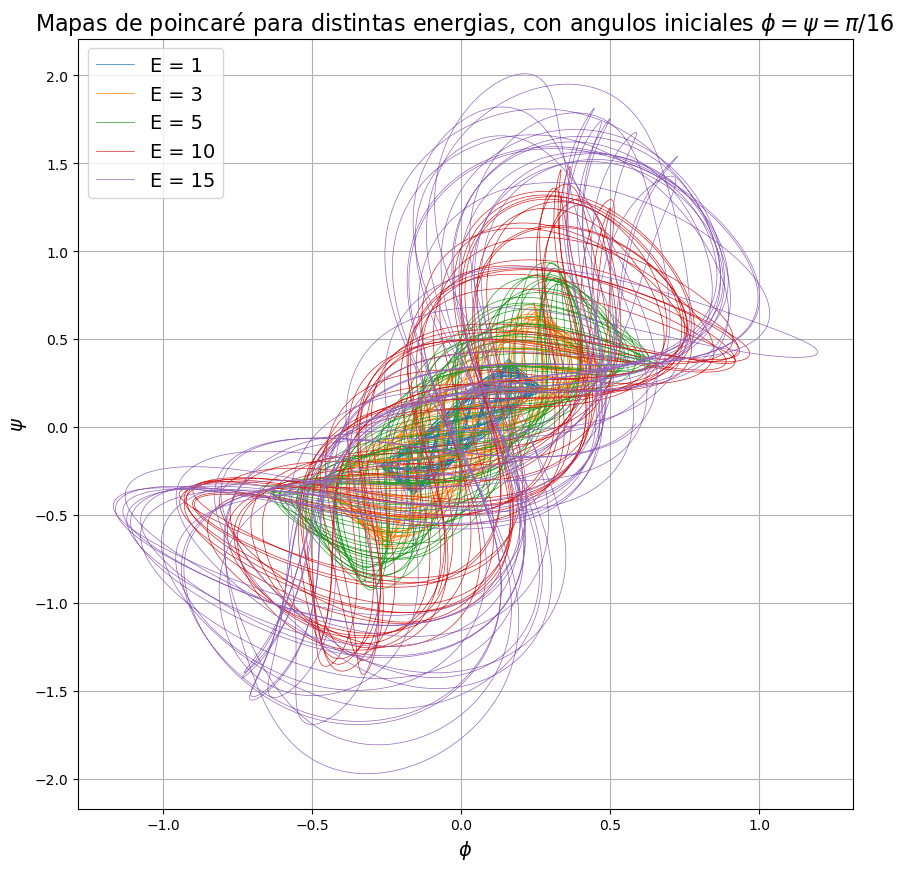
\includegraphics[width=\textwidth]{plots/poincare_energias.png}
    \caption{Mapa de Poincaré para distintas energías}
    \label{fig:poincare_energias}
\end{figure}

Centrandonos en la energía $E = 1$ (figura \ref{fig:poincare_energia_1}) 
se puede observar que el sistema tiende a ciertas configuraciones, 

\begin{figure}
    \centering
    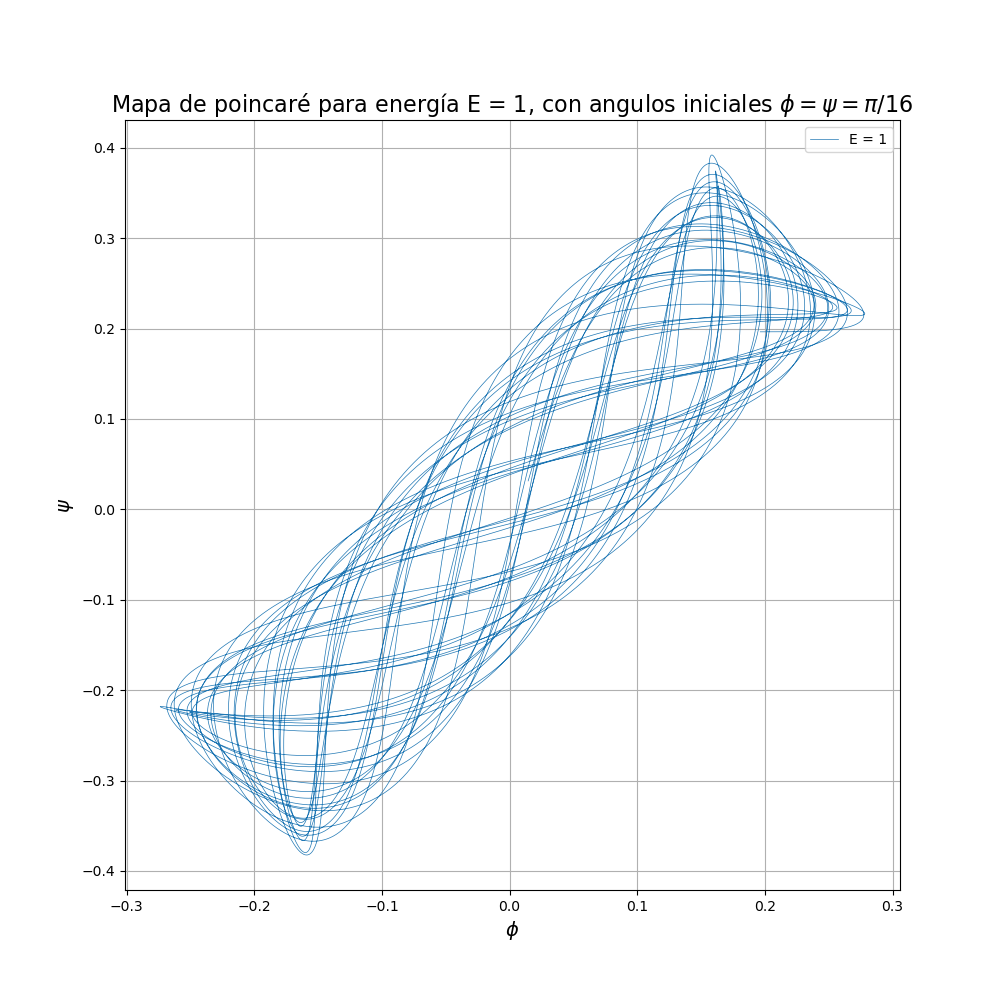
\includegraphics[width=\textwidth]{plots/poincare_energias_1.png}
    \caption{Mapa de Poincaré para E = 1}
    \label{fig:poincare_energia_1}
\end{figure}

Para energías mayores, se va deformando la forma inicial 

A grandes rasgos, se puede observar 


Representado los ángulos con sus velocidades angulares

\begin{figure}
    \centering
    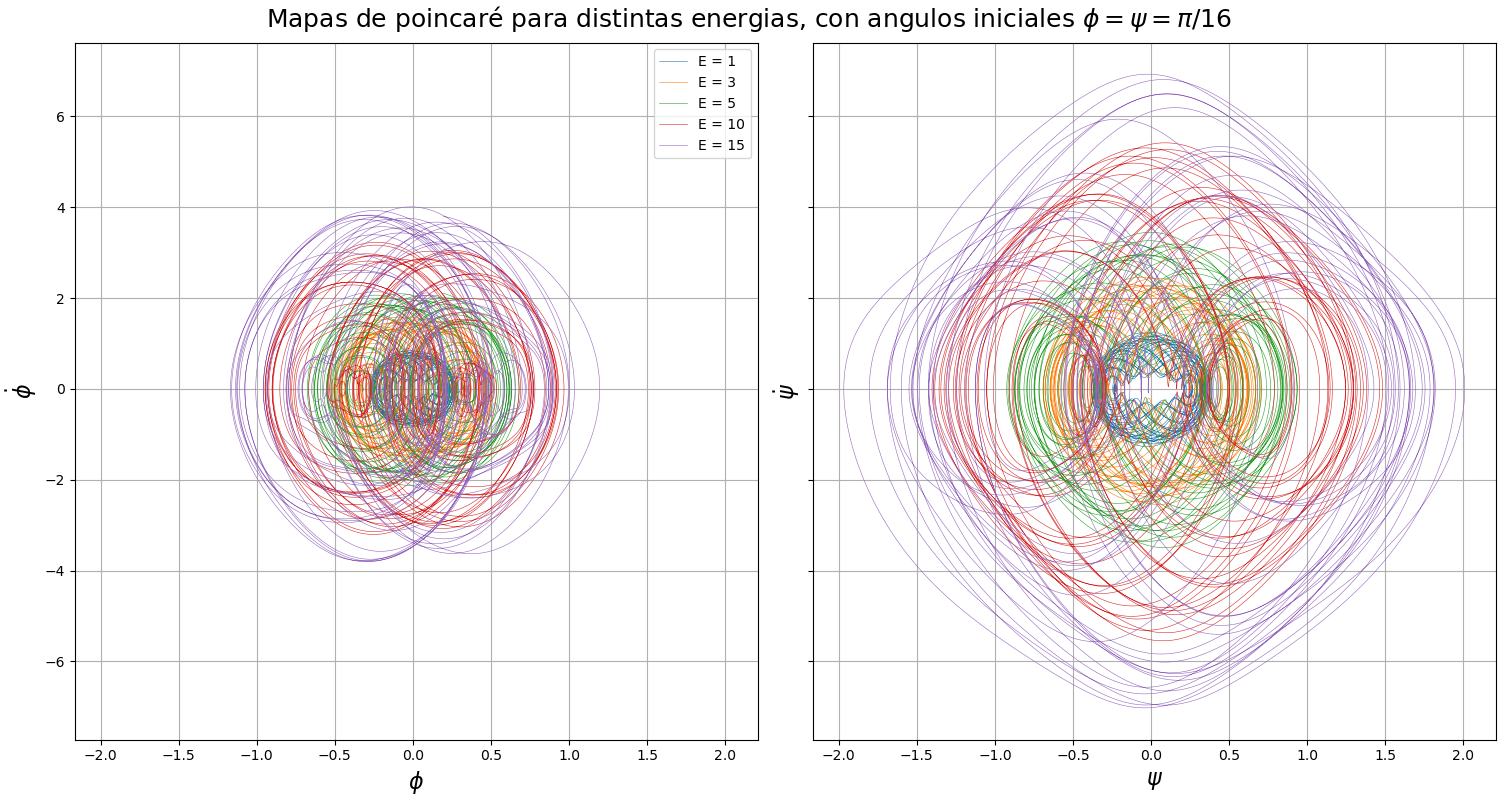
\includegraphics[width=\textwidth]{plots/poincare_energias_phi_psi.png}
    \caption{Relación entre $\phi$ y $\dot{\phi}$}
    \label{fig:poincare_energias_phi}
\end{figure}

\subsection{Coeficiente de Lyapunov}

Para un sistema caótico, el coeficiente de Lyapunov nos permite
cuantificar la tasa de divergencia de dos trayectorias infinitamente
cercanas.

\subsection{Estabilidad del sistema}

\subsection{Optimización}

Se va a comparar el tiempo de ejecución de los métodos de Runge-Kutta, para 
distintas maquinas, distintos tamaños de paso $h$, y distintos tiempo total 
de simulación.

Se ha considerado 3 ordenadores distintos, con las siguientes características:



\newpage

\appendix

\section{Tabla de valores}


\newpage

\section{Análisis de errores}


\end{document}
